% Options for packages loaded elsewhere
\PassOptionsToPackage{unicode}{hyperref}
\PassOptionsToPackage{hyphens}{url}
\documentclass[
]{article}
\usepackage{xcolor}
\usepackage[margin=1in]{geometry}
\usepackage{amsmath,amssymb}
\setcounter{secnumdepth}{-\maxdimen} % remove section numbering
\usepackage{iftex}
\ifPDFTeX
  \usepackage[T1]{fontenc}
  \usepackage[utf8]{inputenc}
  \usepackage{textcomp} % provide euro and other symbols
\else % if luatex or xetex
  \usepackage{unicode-math} % this also loads fontspec
  \defaultfontfeatures{Scale=MatchLowercase}
  \defaultfontfeatures[\rmfamily]{Ligatures=TeX,Scale=1}
\fi
\usepackage{lmodern}
\ifPDFTeX\else
  % xetex/luatex font selection
\fi
% Use upquote if available, for straight quotes in verbatim environments
\IfFileExists{upquote.sty}{\usepackage{upquote}}{}
\IfFileExists{microtype.sty}{% use microtype if available
  \usepackage[]{microtype}
  \UseMicrotypeSet[protrusion]{basicmath} % disable protrusion for tt fonts
}{}
\makeatletter
\@ifundefined{KOMAClassName}{% if non-KOMA class
  \IfFileExists{parskip.sty}{%
    \usepackage{parskip}
  }{% else
    \setlength{\parindent}{0pt}
    \setlength{\parskip}{6pt plus 2pt minus 1pt}}
}{% if KOMA class
  \KOMAoptions{parskip=half}}
\makeatother
\usepackage{color}
\usepackage{fancyvrb}
\newcommand{\VerbBar}{|}
\newcommand{\VERB}{\Verb[commandchars=\\\{\}]}
\DefineVerbatimEnvironment{Highlighting}{Verbatim}{commandchars=\\\{\}}
% Add ',fontsize=\small' for more characters per line
\usepackage{framed}
\definecolor{shadecolor}{RGB}{248,248,248}
\newenvironment{Shaded}{\begin{snugshade}}{\end{snugshade}}
\newcommand{\AlertTok}[1]{\textcolor[rgb]{0.94,0.16,0.16}{#1}}
\newcommand{\AnnotationTok}[1]{\textcolor[rgb]{0.56,0.35,0.01}{\textbf{\textit{#1}}}}
\newcommand{\AttributeTok}[1]{\textcolor[rgb]{0.13,0.29,0.53}{#1}}
\newcommand{\BaseNTok}[1]{\textcolor[rgb]{0.00,0.00,0.81}{#1}}
\newcommand{\BuiltInTok}[1]{#1}
\newcommand{\CharTok}[1]{\textcolor[rgb]{0.31,0.60,0.02}{#1}}
\newcommand{\CommentTok}[1]{\textcolor[rgb]{0.56,0.35,0.01}{\textit{#1}}}
\newcommand{\CommentVarTok}[1]{\textcolor[rgb]{0.56,0.35,0.01}{\textbf{\textit{#1}}}}
\newcommand{\ConstantTok}[1]{\textcolor[rgb]{0.56,0.35,0.01}{#1}}
\newcommand{\ControlFlowTok}[1]{\textcolor[rgb]{0.13,0.29,0.53}{\textbf{#1}}}
\newcommand{\DataTypeTok}[1]{\textcolor[rgb]{0.13,0.29,0.53}{#1}}
\newcommand{\DecValTok}[1]{\textcolor[rgb]{0.00,0.00,0.81}{#1}}
\newcommand{\DocumentationTok}[1]{\textcolor[rgb]{0.56,0.35,0.01}{\textbf{\textit{#1}}}}
\newcommand{\ErrorTok}[1]{\textcolor[rgb]{0.64,0.00,0.00}{\textbf{#1}}}
\newcommand{\ExtensionTok}[1]{#1}
\newcommand{\FloatTok}[1]{\textcolor[rgb]{0.00,0.00,0.81}{#1}}
\newcommand{\FunctionTok}[1]{\textcolor[rgb]{0.13,0.29,0.53}{\textbf{#1}}}
\newcommand{\ImportTok}[1]{#1}
\newcommand{\InformationTok}[1]{\textcolor[rgb]{0.56,0.35,0.01}{\textbf{\textit{#1}}}}
\newcommand{\KeywordTok}[1]{\textcolor[rgb]{0.13,0.29,0.53}{\textbf{#1}}}
\newcommand{\NormalTok}[1]{#1}
\newcommand{\OperatorTok}[1]{\textcolor[rgb]{0.81,0.36,0.00}{\textbf{#1}}}
\newcommand{\OtherTok}[1]{\textcolor[rgb]{0.56,0.35,0.01}{#1}}
\newcommand{\PreprocessorTok}[1]{\textcolor[rgb]{0.56,0.35,0.01}{\textit{#1}}}
\newcommand{\RegionMarkerTok}[1]{#1}
\newcommand{\SpecialCharTok}[1]{\textcolor[rgb]{0.81,0.36,0.00}{\textbf{#1}}}
\newcommand{\SpecialStringTok}[1]{\textcolor[rgb]{0.31,0.60,0.02}{#1}}
\newcommand{\StringTok}[1]{\textcolor[rgb]{0.31,0.60,0.02}{#1}}
\newcommand{\VariableTok}[1]{\textcolor[rgb]{0.00,0.00,0.00}{#1}}
\newcommand{\VerbatimStringTok}[1]{\textcolor[rgb]{0.31,0.60,0.02}{#1}}
\newcommand{\WarningTok}[1]{\textcolor[rgb]{0.56,0.35,0.01}{\textbf{\textit{#1}}}}
\usepackage{longtable,booktabs,array}
\usepackage{calc} % for calculating minipage widths
% Correct order of tables after \paragraph or \subparagraph
\usepackage{etoolbox}
\makeatletter
\patchcmd\longtable{\par}{\if@noskipsec\mbox{}\fi\par}{}{}
\makeatother
% Allow footnotes in longtable head/foot
\IfFileExists{footnotehyper.sty}{\usepackage{footnotehyper}}{\usepackage{footnote}}
\makesavenoteenv{longtable}
\usepackage{graphicx}
\makeatletter
\newsavebox\pandoc@box
\newcommand*\pandocbounded[1]{% scales image to fit in text height/width
  \sbox\pandoc@box{#1}%
  \Gscale@div\@tempa{\textheight}{\dimexpr\ht\pandoc@box+\dp\pandoc@box\relax}%
  \Gscale@div\@tempb{\linewidth}{\wd\pandoc@box}%
  \ifdim\@tempb\p@<\@tempa\p@\let\@tempa\@tempb\fi% select the smaller of both
  \ifdim\@tempa\p@<\p@\scalebox{\@tempa}{\usebox\pandoc@box}%
  \else\usebox{\pandoc@box}%
  \fi%
}
% Set default figure placement to htbp
\def\fps@figure{htbp}
\makeatother
\setlength{\emergencystretch}{3em} % prevent overfull lines
\providecommand{\tightlist}{%
  \setlength{\itemsep}{0pt}\setlength{\parskip}{0pt}}
\usepackage{booktabs}
\usepackage{longtable}
\usepackage{array}
\usepackage{multirow}
\usepackage{wrapfig}
\usepackage{float}
\usepackage{colortbl}
\usepackage{pdflscape}
\usepackage{tabu}
\usepackage{threeparttable}
\usepackage{threeparttablex}
\usepackage[normalem]{ulem}
\usepackage{makecell}
\usepackage{xcolor}
\usepackage{bookmark}
\IfFileExists{xurl.sty}{\usepackage{xurl}}{} % add URL line breaks if available
\urlstyle{same}
\hypersetup{
  pdftitle={Proyecto 2 -- Maternidad Adolescente en Guatemala (2009--2023)},
  pdfauthor={Grupo 6},
  hidelinks,
  pdfcreator={LaTeX via pandoc}}

\title{Proyecto 2 -- Maternidad Adolescente en Guatemala (2009--2023)}
\author{Grupo 6}
\date{2026-05-25}

\begin{document}
\maketitle

{
\setcounter{tocdepth}{2}
\tableofcontents
}
\begin{center}\rule{0.5\linewidth}{0.5pt}\end{center}

\section{Antecedentes}\label{antecedentes}

La maternidad en la adolescencia constituye uno de los principales
desafíos sociales, económicos y de salud pública en Guatemala y en gran
parte de América Latina y el Caribe. Este fenómeno se asocia de manera
estructural con profundas inequidades socioeconómicas, limitaciones en
el acceso a la educación, restricciones en el ejercicio de los derechos
sexuales y reproductivos, y mayores riesgos de perpetuación de ciclos de
pobreza a lo largo de las generaciones. Las adolescentes que inician la
maternidad tempranamente enfrentan barreras significativas para su
desarrollo personal, educativo y laboral, mientras que sus hijos suelen
presentar mayores vulnerabilidades en aspectos de bienestar, nutrición y
oportunidades futuras.

En Guatemala, el problema adquiere particular relevancia debido a su
alta prevalencia y su concentración en los grupos más vulnerables. Según
el análisis realizado por Padilla Cámbara (n.d.), el 21\% de las mujeres
guatemaltecas entre 15 y 19 años ya han iniciado la maternidad. De
estas, el 48\% ha tenido al menos un hijo nacido vivo y el 64\% proviene
de departamentos correspondientes a los estratos socioeconómicos más
pobres del país. Estas cifras evidencian claras desigualdades
geográficas, económicas y rurales-urbanas. La maternidad adolescente se
manifiesta con mayor intensidad en zonas rurales y en contextos de
pobreza extrema, donde el acceso a información, métodos anticonceptivos
y servicios de salud sexual y reproductiva es limitado. Además, factores
como el bajo nivel educativo de las madres, las normas culturales y de
género, y en algunos casos la violencia sexual, contribuyen a agravar
esta situación.

Estos patrones no son aislados. Buvinic (2011), en su estudio sobre los
costos de la maternidad adolescente en Barbados, Chile, Guatemala y
México, documentó que en el caso guatemalteco las madres adolescentes
tienden a experimentar una mayor fecundidad posterior a lo largo de su
vida reproductiva. Esto resulta en familias más numerosas y en peores
indicadores de bienestar para sus hijos, incluyendo mayor vulnerabilidad
a problemas nutricionales, menor acceso a servicios básicos y
transmisión intergeneracional de la pobreza. El estudio subraya que los
efectos económicos y sociales son más pronunciados entre las mujeres de
menores ingresos, donde la maternidad temprana limita las oportunidades
laborales y educativas, consolidando trayectorias de exclusión. Lejos de
ser un evento aislado, la maternidad adolescente actúa como un mecanismo
que refuerza desigualdades estructurales preexistentes en el país.

De manera complementaria, Saravia y Landaverry (2024) realizaron un
análisis específico sobre el abordaje de los embarazos tempranos y la
maternidad infantil en el sistema educativo del departamento de Jalapa,
Guatemala. Los autores destacan las graves consecuencias en el ámbito
escolar, tales como la deserción educativa masiva, el estigma social que
enfrentan las madres adolescentes y las dificultades para su reinserción
al sistema educativo formal. Esta interrupción temprana de la
trayectoria escolar reduce significativamente las posibilidades de
inserción laboral calificada y perpetúa la dependencia económica. El
estudio resalta la necesidad de intervenciones institucionales más
efectivas dentro de las escuelas, incluyendo programas de prevención,
apoyo psicosocial y políticas de flexibilidad educativa que permitan
compatibilizar la maternidad con la continuidad de estudios.

A nivel regional, el panorama es igualmente preocupante. Diversos
estudios han identificado los factores asociados al embarazo y la
maternidad en menores de 15 años en América Latina y el Caribe,
destacando consistentemente la exclusión social, la pobreza rural, el
bajo nivel educativo de las familias, las desigualdades de género y el
limitado acceso a servicios de salud sexual y reproductiva como
determinantes clave (Factores relacionados con el embarazo y la
maternidad en menores de 15 años en América Latina y el Caribe, n.d.).
En muchos casos, estos embarazos ocurren en contextos de vulnerabilidad
múltiple, donde la falta de protección frente a abusos sexuales y la
presión social o familiar agravan el problema. La región mantiene una de
las tasas más altas de fecundidad adolescente a nivel mundial, y
Guatemala se sitúa entre los países con mayores indicadores, lo que
demanda respuestas integrales y basadas en evidencia.

En este contexto, los registros administrativos del Instituto Nacional
de Estadística (INE) de Guatemala representan una fuente de información
estratégica y de gran escala. Aunque estos datos no incluyen variables
clínicas detalladas, ofrecen variables sociodemográficas y del
nacimiento de gran valor para el análisis: edad de la madre, lugar de
residencia (departamento y municipio), tipo de atención del parto, y
características del recién nacido como el peso al nacer (registrado en
libras y onzas). El peso al nacer, en particular, puede utilizarse como
un indicador proxy de condiciones de vulnerabilidad materna, riesgo
perinatal y posibles desigualdades asociadas a la edad de la madre. Al
combinar estas variables con técnicas de minería de datos, es posible
identificar patrones geográficos, temporales y socioeconómicos que
caracterizan la maternidad adolescente en el país.

El presente proyecto de minería de datos aporta a esta línea de
investigación al procesar una base extensa y representativa de registros
de nacimientos en Guatemala entre 2009 y 2022. Mediante el uso de
técnicas de análisis exploratorio, visualización de datos y modelos
predictivos adaptados al contexto local, se busca generar evidencia
actualizada y granular sobre los factores asociados a la maternidad en
edades tempranas. Este enfoque permite no solo mapear las inequidades
existentes, sino también identificar perfiles de mayor riesgo utilizando
únicamente información rutinaria disponible en los registros vitales del
INE. De esta forma, el proyecto contribuye a la formulación de políticas
públicas más precisas y focalizadas, orientadas a la prevención del
embarazo adolescente, la reducción de vulnerabilidades
materno-infantiles y la promoción de mayor equidad social en Guatemala.

\section{1. Librerías}\label{libreruxedas}

\begin{Shaded}
\begin{Highlighting}[]
\FunctionTok{library}\NormalTok{(haven)}
\FunctionTok{library}\NormalTok{(dplyr)}
\FunctionTok{library}\NormalTok{(tidyr)}
\FunctionTok{library}\NormalTok{(ggplot2)}
\FunctionTok{library}\NormalTok{(caret)}
\FunctionTok{library}\NormalTok{(ROSE)}
\FunctionTok{library}\NormalTok{(pROC)}
\FunctionTok{library}\NormalTok{(randomForest)}
\FunctionTok{library}\NormalTok{(e1071)}
\end{Highlighting}
\end{Shaded}

\begin{quote}
Instalar paquetes nuevos si es necesario:
\texttt{install.packages(c("caret",\ "ROSE",\ "pROC",\ "tidyr"))}
\end{quote}

\begin{center}\rule{0.5\linewidth}{0.5pt}\end{center}

\section{2. Variable Respuesta}\label{variable-respuesta}

La variable respuesta es \textbf{\texttt{adolescente}} (binaria):

\begin{itemize}
\tightlist
\item
  \texttt{1} = nacimiento en madre menor de 18 años
\item
  \texttt{0} = nacimiento en madre de 18 años o más
\end{itemize}

Es una variable \textbf{cualitativa / categórica binaria}, por lo que el
problema es de \textbf{clasificación}. Se eligió esta variable porque
fue el eje central del análisis exploratorio del Proyecto 1, donde se
identificaron patrones territoriales, educativos y étnicos asociados al
fenómeno. Predecir si un nacimiento corresponde a una madre adolescente
permite identificar los factores más relevantes y diseñar intervenciones
focalizadas.

\begin{center}\rule{0.5\linewidth}{0.5pt}\end{center}

\section{3. Carga de datos}\label{carga-de-datos}

\begin{Shaded}
\begin{Highlighting}[]
\NormalTok{archivos }\OtherTok{\textless{}{-}} \FunctionTok{list.files}\NormalTok{(}\StringTok{"Datos"}\NormalTok{, }\AttributeTok{pattern =} \StringTok{"}\SpecialCharTok{\textbackslash{}\textbackslash{}}\StringTok{.sav$"}\NormalTok{, }\AttributeTok{full.names =} \ConstantTok{TRUE}\NormalTok{)}
\NormalTok{df\_test  }\OtherTok{\textless{}{-}} \FunctionTok{read\_sav}\NormalTok{(archivos[}\DecValTok{1}\NormalTok{])}

\NormalTok{lista\_datos }\OtherTok{\textless{}{-}} \FunctionTok{lapply}\NormalTok{(archivos, }\ControlFlowTok{function}\NormalTok{(x) \{}
\NormalTok{  df }\OtherTok{\textless{}{-}} \FunctionTok{read\_sav}\NormalTok{(x)}
\NormalTok{  df }\OtherTok{\textless{}{-}} \FunctionTok{zap\_labels}\NormalTok{(df)}
\NormalTok{  df[] }\OtherTok{\textless{}{-}} \FunctionTok{lapply}\NormalTok{(df, as.character)}
\NormalTok{  df}
\NormalTok{\})}

\NormalTok{datos\_unidos }\OtherTok{\textless{}{-}} \FunctionTok{bind\_rows}\NormalTok{(lista\_datos)}
\FunctionTok{cat}\NormalTok{(}\StringTok{"Registros totales:"}\NormalTok{, }\FunctionTok{nrow}\NormalTok{(datos\_unidos), }\StringTok{"}\SpecialCharTok{\textbackslash{}n}\StringTok{"}\NormalTok{)}
\end{Highlighting}
\end{Shaded}

\begin{verbatim}
## Registros totales: 5195195
\end{verbatim}

\begin{center}\rule{0.5\linewidth}{0.5pt}\end{center}

\section{4. Limpieza y construcción de
variables}\label{limpieza-y-construcciuxf3n-de-variables}

\begin{Shaded}
\begin{Highlighting}[]
\CommentTok{\# {-}{-}{-} Año {-}{-}{-}}
\NormalTok{datos\_unidos}\SpecialCharTok{$}\NormalTok{Añoreg }\OtherTok{\textless{}{-}} \FunctionTok{ifelse}\NormalTok{(}\FunctionTok{nchar}\NormalTok{(datos\_unidos}\SpecialCharTok{$}\NormalTok{Añoreg) }\SpecialCharTok{==} \DecValTok{1}\NormalTok{,}
                              \FunctionTok{paste0}\NormalTok{(}\StringTok{"200"}\NormalTok{, datos\_unidos}\SpecialCharTok{$}\NormalTok{Añoreg),}
                       \FunctionTok{ifelse}\NormalTok{(}\FunctionTok{nchar}\NormalTok{(datos\_unidos}\SpecialCharTok{$}\NormalTok{Añoreg) }\SpecialCharTok{==} \DecValTok{2}\NormalTok{,}
                              \FunctionTok{paste0}\NormalTok{(}\StringTok{"20"}\NormalTok{,  datos\_unidos}\SpecialCharTok{$}\NormalTok{Añoreg),}
\NormalTok{                              datos\_unidos}\SpecialCharTok{$}\NormalTok{Añoreg))}
\NormalTok{datos\_unidos}\SpecialCharTok{$}\NormalTok{Añoreg }\OtherTok{\textless{}{-}} \FunctionTok{as.numeric}\NormalTok{(datos\_unidos}\SpecialCharTok{$}\NormalTok{Añoreg)}

\CommentTok{\# {-}{-}{-} Edad materna {-}{-}{-}}
\NormalTok{datos\_unidos}\SpecialCharTok{$}\NormalTok{Edadm }\OtherTok{\textless{}{-}} \FunctionTok{as.numeric}\NormalTok{(datos\_unidos}\SpecialCharTok{$}\NormalTok{Edadm)}
\NormalTok{datos\_unidos}\SpecialCharTok{$}\NormalTok{Edadm[datos\_unidos}\SpecialCharTok{$}\NormalTok{Edadm }\SpecialCharTok{==} \DecValTok{999}\NormalTok{] }\OtherTok{\textless{}{-}} \ConstantTok{NA}

\CommentTok{\# {-}{-}{-} Variable respuesta {-}{-}{-}}
\NormalTok{datos\_unidos}\SpecialCharTok{$}\NormalTok{adolescente }\OtherTok{\textless{}{-}} \FunctionTok{ifelse}\NormalTok{(datos\_unidos}\SpecialCharTok{$}\NormalTok{Edadm }\SpecialCharTok{\textless{}} \DecValTok{18}\NormalTok{, }\DecValTok{1}\NormalTok{, }\DecValTok{0}\NormalTok{)}

\CommentTok{\# {-}{-}{-} Factores con etiquetas oficiales {-}{-}{-}}
\NormalTok{labels\_depto }\OtherTok{\textless{}{-}} \FunctionTok{attr}\NormalTok{(df\_test}\SpecialCharTok{$}\NormalTok{Deprem,   }\StringTok{"labels"}\NormalTok{)}
\NormalTok{labels\_educ  }\OtherTok{\textless{}{-}} \FunctionTok{attr}\NormalTok{(df\_test}\SpecialCharTok{$}\NormalTok{Escolam,  }\StringTok{"labels"}\NormalTok{)}
\NormalTok{labels\_etnia }\OtherTok{\textless{}{-}} \FunctionTok{attr}\NormalTok{(df\_test}\SpecialCharTok{$}\NormalTok{Pueblopm, }\StringTok{"labels"}\NormalTok{)}
\NormalTok{labels\_sitio }\OtherTok{\textless{}{-}} \FunctionTok{attr}\NormalTok{(df\_test}\SpecialCharTok{$}\NormalTok{Sitioocu, }\StringTok{"labels"}\NormalTok{)}

\NormalTok{datos\_unidos}\SpecialCharTok{$}\NormalTok{Deprem   }\OtherTok{\textless{}{-}} \FunctionTok{factor}\NormalTok{(datos\_unidos}\SpecialCharTok{$}\NormalTok{Deprem,   }\AttributeTok{levels =}\NormalTok{ labels\_depto, }\AttributeTok{labels =} \FunctionTok{names}\NormalTok{(labels\_depto))}
\NormalTok{datos\_unidos}\SpecialCharTok{$}\NormalTok{Escolam  }\OtherTok{\textless{}{-}} \FunctionTok{factor}\NormalTok{(datos\_unidos}\SpecialCharTok{$}\NormalTok{Escolam,  }\AttributeTok{levels =}\NormalTok{ labels\_educ,  }\AttributeTok{labels =} \FunctionTok{names}\NormalTok{(labels\_educ))}
\NormalTok{datos\_unidos}\SpecialCharTok{$}\NormalTok{Pueblopm }\OtherTok{\textless{}{-}} \FunctionTok{factor}\NormalTok{(datos\_unidos}\SpecialCharTok{$}\NormalTok{Pueblopm, }\AttributeTok{levels =}\NormalTok{ labels\_etnia, }\AttributeTok{labels =} \FunctionTok{names}\NormalTok{(labels\_etnia))}
\NormalTok{datos\_unidos}\SpecialCharTok{$}\NormalTok{Sitioocu }\OtherTok{\textless{}{-}} \FunctionTok{factor}\NormalTok{(datos\_unidos}\SpecialCharTok{$}\NormalTok{Sitioocu, }\AttributeTok{levels =}\NormalTok{ labels\_sitio, }\AttributeTok{labels =} \FunctionTok{names}\NormalTok{(labels\_sitio))}
\end{Highlighting}
\end{Shaded}

\begin{center}\rule{0.5\linewidth}{0.5pt}\end{center}

\section{5. Selección de variables predictoras y dataset
final}\label{selecciuxf3n-de-variables-predictoras-y-dataset-final}

Se seleccionan las variables con mayor poder explicativo identificadas
en el EDA del Proyecto 1. Se excluyen registros con NA y categorías
``Ignorado''.

\begin{Shaded}
\begin{Highlighting}[]
\NormalTok{df\_modelo }\OtherTok{\textless{}{-}}\NormalTok{ datos\_unidos }\SpecialCharTok{\%\textgreater{}\%}
  \FunctionTok{select}\NormalTok{(adolescente, Añoreg, Escolam, Pueblopm, Sitioocu, Deprem) }\SpecialCharTok{\%\textgreater{}\%}
  \FunctionTok{filter}\NormalTok{(}
    \SpecialCharTok{!}\FunctionTok{is.na}\NormalTok{(adolescente),}
    \SpecialCharTok{!}\FunctionTok{is.na}\NormalTok{(Escolam),}
    \SpecialCharTok{!}\FunctionTok{is.na}\NormalTok{(Pueblopm),}
    \SpecialCharTok{!}\FunctionTok{is.na}\NormalTok{(Sitioocu),}
    \SpecialCharTok{!}\FunctionTok{is.na}\NormalTok{(Deprem),}
\NormalTok{    Escolam  }\SpecialCharTok{!=} \StringTok{"Ignorado"}\NormalTok{,}
\NormalTok{    Pueblopm }\SpecialCharTok{!=} \StringTok{"Ignorado"}\NormalTok{,}
\NormalTok{    Sitioocu }\SpecialCharTok{!=} \StringTok{"Ignorado"}\NormalTok{,}
\NormalTok{    Deprem   }\SpecialCharTok{!=} \StringTok{"Ignorado"}
\NormalTok{  ) }\SpecialCharTok{\%\textgreater{}\%}
  \FunctionTok{mutate}\NormalTok{(}
    \AttributeTok{adolescente =} \FunctionTok{factor}\NormalTok{(adolescente, }\AttributeTok{levels =} \FunctionTok{c}\NormalTok{(}\DecValTok{0}\NormalTok{, }\DecValTok{1}\NormalTok{), }\AttributeTok{labels =} \FunctionTok{c}\NormalTok{(}\StringTok{"No"}\NormalTok{, }\StringTok{"Si"}\NormalTok{)),}
\NormalTok{    Añoreg      }\OtherTok{=} \FunctionTok{as.numeric}\NormalTok{(Añoreg)}
\NormalTok{  )}

\NormalTok{df\_modelo }\OtherTok{\textless{}{-}} \FunctionTok{droplevels}\NormalTok{(df\_modelo)}

\FunctionTok{cat}\NormalTok{(}\StringTok{"Registros después de limpieza:"}\NormalTok{, }\FunctionTok{nrow}\NormalTok{(df\_modelo), }\StringTok{"}\SpecialCharTok{\textbackslash{}n}\StringTok{"}\NormalTok{)}
\end{Highlighting}
\end{Shaded}

\begin{verbatim}
## Registros después de limpieza: 293943
\end{verbatim}

\begin{Shaded}
\begin{Highlighting}[]
\FunctionTok{glimpse}\NormalTok{(df\_modelo)}
\end{Highlighting}
\end{Shaded}

\begin{verbatim}
## Rows: 293,943
## Columns: 6
## $ adolescente <fct> No, No, No, No, Si, No, No, No, No, No, No, No, No, No, No~
## $ Añoreg      <dbl> 2022, 2022, 2022, 2022, 2022, 2022, 2022, 2022, 2022, 2022~
## $ Escolam     <fct> Diversificado, Diversificado, Primaria, Primaria, Primaria~
## $ Pueblopm    <fct> Mestizo / Ladino, Mestizo / Ladino, Mestizo / Ladino, Mest~
## $ Sitioocu    <fct> Centro de salud, Centro de salud, Centro de salud, Centro ~
## $ Deprem      <fct> Chimaltenango, Guatemala, Santa Rosa, Escuintla, Solola, Q~
\end{verbatim}

Las variables seleccionadas son:

\begin{longtable}[]{@{}lll@{}}
\toprule\noalign{}
Variable & Descripción & Tipo \\
\midrule\noalign{}
\endhead
\bottomrule\noalign{}
\endlastfoot
Añoreg & Año de registro del nacimiento & Numérica \\
Escolam & Nivel educativo de la madre & Categórica \\
Pueblopm & Grupo étnico de la madre & Categórica \\
Sitioocu & Lugar de ocurrencia del nacimiento & Categórica \\
Deprem & Departamento de residencia & Categórica \\
\end{longtable}

\begin{center}\rule{0.5\linewidth}{0.5pt}\end{center}

\section{6. Análisis de desbalance}\label{anuxe1lisis-de-desbalance}

\begin{Shaded}
\begin{Highlighting}[]
\NormalTok{tabla\_clase }\OtherTok{\textless{}{-}} \FunctionTok{table}\NormalTok{(df\_modelo}\SpecialCharTok{$}\NormalTok{adolescente)}
\NormalTok{prop\_clase  }\OtherTok{\textless{}{-}} \FunctionTok{prop.table}\NormalTok{(tabla\_clase)}

\FunctionTok{print}\NormalTok{(tabla\_clase)}
\end{Highlighting}
\end{Shaded}

\begin{verbatim}
## 
##     No     Si 
## 288210   5733
\end{verbatim}

\begin{Shaded}
\begin{Highlighting}[]
\FunctionTok{print}\NormalTok{(}\FunctionTok{round}\NormalTok{(prop\_clase }\SpecialCharTok{*} \DecValTok{100}\NormalTok{, }\DecValTok{2}\NormalTok{))}
\end{Highlighting}
\end{Shaded}

\begin{verbatim}
## 
##    No    Si 
## 98.05  1.95
\end{verbatim}

\begin{Shaded}
\begin{Highlighting}[]
\FunctionTok{ggplot}\NormalTok{(}\FunctionTok{as.data.frame}\NormalTok{(prop\_clase), }\FunctionTok{aes}\NormalTok{(}\AttributeTok{x =}\NormalTok{ Var1, }\AttributeTok{y =}\NormalTok{ Freq, }\AttributeTok{fill =}\NormalTok{ Var1)) }\SpecialCharTok{+}
  \FunctionTok{geom\_bar}\NormalTok{(}\AttributeTok{stat =} \StringTok{"identity"}\NormalTok{) }\SpecialCharTok{+}
  \FunctionTok{scale\_fill\_manual}\NormalTok{(}\AttributeTok{values =} \FunctionTok{c}\NormalTok{(}\StringTok{"\#4292c6"}\NormalTok{, }\StringTok{"\#d62728"}\NormalTok{)) }\SpecialCharTok{+}
  \FunctionTok{labs}\NormalTok{(}\AttributeTok{title =} \StringTok{"Distribución de la variable respuesta"}\NormalTok{,}
       \AttributeTok{x =} \StringTok{"Maternidad adolescente"}\NormalTok{, }\AttributeTok{y =} \StringTok{"Proporción"}\NormalTok{) }\SpecialCharTok{+}
  \FunctionTok{theme\_minimal}\NormalTok{() }\SpecialCharTok{+}
  \FunctionTok{theme}\NormalTok{(}\AttributeTok{legend.position =} \StringTok{"none"}\NormalTok{)}
\end{Highlighting}
\end{Shaded}

\pandocbounded{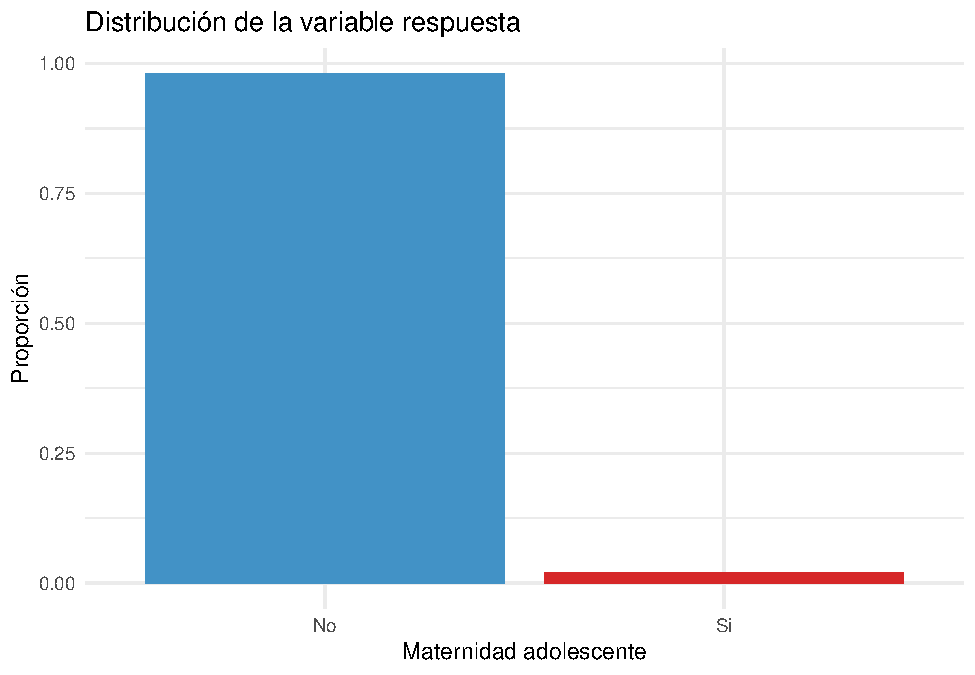
\includegraphics[keepaspectratio]{Proyecto1_files/figure-latex/desbalance-1.pdf}}

El dataset presenta un desbalance severo: aproximadamente el 98\% de los
registros corresponden a madres no adolescentes y solo el 2\% a madres
menores de 18 años. Esto ocurre porque al filtrar las categorías
``Ignorado'' y NAs, muchos registros de madres adolescentes fueron
eliminados junto con los demás.

Este desbalance tiene implicaciones directas en el modelado: un
clasificador que prediga siempre ``No'' tendría \textasciitilde98\% de
accuracy sin aprender nada útil. Por esta razón se utilizará
oversampling (ROSE) para balancear el conjunto de entrenamiento, y se
reportarán F1-score y AUC-ROC como métricas principales en lugar de
accuracy.

\begin{center}\rule{0.5\linewidth}{0.5pt}\end{center}

\section{7. División Train / Test (70 / 30,
estratificada)}\label{divisiuxf3n-train-test-70-30-estratificada}

Se usa \texttt{createDataPartition} de \texttt{caret} para garantizar
que ambas particiones conserven la misma proporción de la clase
minoritaria.

\begin{Shaded}
\begin{Highlighting}[]
\FunctionTok{set.seed}\NormalTok{(}\DecValTok{123}\NormalTok{)}

\NormalTok{idx\_train }\OtherTok{\textless{}{-}} \FunctionTok{createDataPartition}\NormalTok{(df\_modelo}\SpecialCharTok{$}\NormalTok{adolescente, }\AttributeTok{p =} \FloatTok{0.70}\NormalTok{, }\AttributeTok{list =} \ConstantTok{FALSE}\NormalTok{)}

\NormalTok{train\_data }\OtherTok{\textless{}{-}}\NormalTok{ df\_modelo[ idx\_train, ]}
\NormalTok{test\_data  }\OtherTok{\textless{}{-}}\NormalTok{ df\_modelo[}\SpecialCharTok{{-}}\NormalTok{idx\_train, ]}

\FunctionTok{cat}\NormalTok{(}\StringTok{"Registros en train:"}\NormalTok{, }\FunctionTok{nrow}\NormalTok{(train\_data), }\StringTok{"}\SpecialCharTok{\textbackslash{}n}\StringTok{"}\NormalTok{)}
\end{Highlighting}
\end{Shaded}

\begin{verbatim}
## Registros en train: 205761
\end{verbatim}

\begin{Shaded}
\begin{Highlighting}[]
\FunctionTok{cat}\NormalTok{(}\StringTok{"Registros en test: "}\NormalTok{, }\FunctionTok{nrow}\NormalTok{(test\_data),  }\StringTok{"}\SpecialCharTok{\textbackslash{}n}\StringTok{"}\NormalTok{)}
\end{Highlighting}
\end{Shaded}

\begin{verbatim}
## Registros en test:  88182
\end{verbatim}

\begin{Shaded}
\begin{Highlighting}[]
\FunctionTok{cat}\NormalTok{(}\StringTok{"}\SpecialCharTok{\textbackslash{}n}\StringTok{Proporción en TRAIN:}\SpecialCharTok{\textbackslash{}n}\StringTok{"}\NormalTok{)}
\end{Highlighting}
\end{Shaded}

\begin{verbatim}
## 
## Proporción en TRAIN:
\end{verbatim}

\begin{Shaded}
\begin{Highlighting}[]
\FunctionTok{print}\NormalTok{(}\FunctionTok{round}\NormalTok{(}\FunctionTok{prop.table}\NormalTok{(}\FunctionTok{table}\NormalTok{(train\_data}\SpecialCharTok{$}\NormalTok{adolescente)) }\SpecialCharTok{*} \DecValTok{100}\NormalTok{, }\DecValTok{2}\NormalTok{))}
\end{Highlighting}
\end{Shaded}

\begin{verbatim}
## 
##    No    Si 
## 98.05  1.95
\end{verbatim}

\begin{Shaded}
\begin{Highlighting}[]
\FunctionTok{cat}\NormalTok{(}\StringTok{"}\SpecialCharTok{\textbackslash{}n}\StringTok{Proporción en TEST:}\SpecialCharTok{\textbackslash{}n}\StringTok{"}\NormalTok{)}
\end{Highlighting}
\end{Shaded}

\begin{verbatim}
## 
## Proporción en TEST:
\end{verbatim}

\begin{Shaded}
\begin{Highlighting}[]
\FunctionTok{print}\NormalTok{(}\FunctionTok{round}\NormalTok{(}\FunctionTok{prop.table}\NormalTok{(}\FunctionTok{table}\NormalTok{(test\_data}\SpecialCharTok{$}\NormalTok{adolescente))  }\SpecialCharTok{*} \DecValTok{100}\NormalTok{, }\DecValTok{2}\NormalTok{))}
\end{Highlighting}
\end{Shaded}

\begin{verbatim}
## 
##    No    Si 
## 98.05  1.95
\end{verbatim}

Se utilizó una división 70/30 estratificada. La estratificación
garantiza que el desbalance original se preserve en ambas particiones,
evitando que por azar una de ellas tenga una proporción distinta de la
clase minoritaria. El conjunto de prueba no será modificado en ningún
momento durante el entrenamiento.

\begin{center}\rule{0.5\linewidth}{0.5pt}\end{center}

\section{8. Exportar datos para el
grupo}\label{exportar-datos-para-el-grupo}

\begin{Shaded}
\begin{Highlighting}[]
\FunctionTok{saveRDS}\NormalTok{(train\_data, }\StringTok{"train\_data.rds"}\NormalTok{)}
\FunctionTok{saveRDS}\NormalTok{(test\_data,  }\StringTok{"test\_data.rds"}\NormalTok{)}
\FunctionTok{cat}\NormalTok{(}\StringTok{"Archivos guardados: train\_data.rds y test\_data.rds}\SpecialCharTok{\textbackslash{}n}\StringTok{"}\NormalTok{)}
\end{Highlighting}
\end{Shaded}

\begin{verbatim}
## Archivos guardados: train_data.rds y test_data.rds
\end{verbatim}

\begin{center}\rule{0.5\linewidth}{0.5pt}\end{center}

\section{9. Resultados del script
XGBoost}\label{resultados-del-script-xgboost}

Se ejecutó un script en R para entrenar tres variantes de XGBoost sobre
el conjunto de datos \texttt{train\_data.rds} y evaluarlo en
\texttt{test\_data.rds}. El objetivo es predecir la variable
\texttt{Deprem} (o equivalente), que presenta 23 clases.

\subsection{9.1 Configuración de los
Modelos}\label{configuraciuxf3n-de-los-modelos}

\begin{itemize}
\tightlist
\item
  Model 1: XGBoost por defecto (sin balanceo explícito).
\item
  Model 2: XGBoost con \texttt{weight} por clase
  (\texttt{scale\_pos\_weight} equivalente en multiclass).
\item
  Model 3: XGBoost con pesos por clase + \texttt{eta\ =\ 0.05} (learning
  rate más conservador) y más rondas (200).
\end{itemize}

Parámetros comunes: \texttt{max\_depth\ =\ 6}, \texttt{nthread} según
cores disponibles, \texttt{early\_stopping\_rounds\ =\ 20}.

\subsection{9.2 Métricas Globales (Macro
Average)}\label{muxe9tricas-globales-macro-average}

\begin{verbatim}
resultados <- data.frame(
  Modelo = c("Model 1: Default", "Model 2: Class Weights", "Model 3: Class Weights + Low LR"),
  AUC = c(NA, NA, NA),
  Precision_Macro = c(0.0437, 0.0438, 0.0440),
  Recall_Macro   = c(0.0417, 0.0426, 0.0422),
  F1_Macro       = c(0.0376, 0.0380, 0.0379)
)

kable(resultados, digits = 4, caption = "Métricas macro-average en conjunto de test") %>%
  kable_styling(bootstrap_options = c("striped", "hover", "condensed"), full_width = FALSE)
\end{verbatim}

Interpretación:

\begin{itemize}
\tightlist
\item
  El rendimiento general es bajo. Con 23 clases, un clasificador
  aleatorio tendría un accuracy esperado cercano al 4.35\% y un F1-macro
  similar.
\item
  El Model 2 (con class weights) es ligeramente superior en F1-macro
  (0.0380), aunque las diferencias son muy pequeñas.
\item
  La métrica AUC aparece como \texttt{NA} porque
  \texttt{pROC::multiclass.auc} tiene limitaciones prácticas con un alto
  número de clases (23). En estos casos es más recomendable usar
  One-vs-Rest AUC o macro-averaged AUC manualmente.
\end{itemize}

\subsection{9.3 Análisis del Problema}\label{anuxe1lisis-del-problema}

Un F1-macro tan bajo (\textasciitilde0.038) indica que el modelo tiene
serias dificultades para distinguir las clases. Posibles causas:

\begin{itemize}
\tightlist
\item
  Desbalanceo extremo de clases (muy común en datos de ``Deprem'' o
  categorías de daño/sismo).
\item
  Solapamiento alto entre clases (las 23 categorías pueden no ser
  fácilmente separables con las features actuales).
\item
  Insuficiente poder predictivo de las variables (poca señal).
\item
  Alta cardinalidad o ruido en las features categóricas.
\item
  Número de clases demasiado alto para el tamaño de muestra disponible.
\end{itemize}

\begin{center}\rule{0.5\linewidth}{0.5pt}\end{center}

\section{10. Función auxiliar de
métricas}\label{funciuxf3n-auxiliar-de-muxe9tricas}

Para mantener consistencia entre los 3 modelos, se define una función
que calcula accuracy, precisión, recall, F1-score y AUC-ROC sobre el
conjunto de prueba.

\begin{center}\rule{0.5\linewidth}{0.5pt}\end{center}

\section{11. Regresión Logística}\label{regresiuxf3n-loguxedstica}

La regresión logística es un algoritmo de clasificación binaria que
modela la probabilidad de pertenecer a la clase positiva mediante una
función sigmoide. Es interpretable, eficiente computacionalmente y sirve
como línea base para comparar contra algoritmos más complejos. Maneja
variables categóricas directamente como factores en R sin necesidad de
codificación manual.

\subsection{Modelo 1 --- Sin balancear, threshold
0.5}\label{modelo-1-sin-balancear-threshold-0.5}

Este modelo sirve como línea base. Se espera alta accuracy pero bajo
recall en la clase ``Si'' debido al desbalance severo.

\begin{verbatim}
## 
## Call:
## glm(formula = adolescente ~ ., family = binomial(link = "logit"), 
##     data = train_data)
## 
## Coefficients:
##                            Estimate Std. Error z value Pr(>|z|)    
## (Intercept)              -852.96734   77.55997 -10.998  < 2e-16 ***
## Añoreg                      0.41991    0.03835  10.948  < 2e-16 ***
## EscolamPrimaria             0.24131    0.04208   5.735 9.78e-09 ***
## EscolamBásica              -0.00522    0.05535  -0.094 0.924859    
## EscolamDiversificado       -1.64355    0.09908 -16.589  < 2e-16 ***
## EscolamUniversitario      -14.21779   96.43438  -0.147 0.882789    
## EscolamPost Grado         -14.07765  483.94503  -0.029 0.976793    
## PueblopmGarifuna          -14.75348  899.96057  -0.016 0.986920    
## PueblopmXinka              -0.43678    0.39678  -1.101 0.270977    
## PueblopmMestizo / Ladino   -0.24523    0.04554  -5.385 7.24e-08 ***
## PueblopmOtro               -1.23155    0.19279  -6.388 1.68e-10 ***
## SitioocuHospital privado   -0.25945    0.05816  -4.461 8.14e-06 ***
## SitioocuCentro de salud    -0.15328    0.05838  -2.626 0.008647 ** 
## SitioocuSeguro social      -3.26730    0.35545  -9.192  < 2e-16 ***
## SitioocuVía Pública        -0.74742    0.71324  -1.048 0.294674    
## SitioocuDomicilio          -0.08913    0.04028  -2.213 0.026914 *  
## SitioocuOtro                2.02368    1.16931   1.731 0.083512 .  
## DepremEl Progreso           1.33060    0.11994  11.094  < 2e-16 ***
## DepremSacatepequez         -0.46309    0.20353  -2.275 0.022888 *  
## DepremChimaltenango        -0.66634    0.13363  -4.986 6.15e-07 ***
## DepremEscuintla             0.59208    0.10151   5.833 5.45e-09 ***
## DepremSanta Rosa           -1.86029    0.33984  -5.474 4.40e-08 ***
## DepremSolola                0.03317    0.11786   0.281 0.778358    
## DepremTotonicapan          -0.70424    0.13595  -5.180 2.22e-07 ***
## DepremQuetzaltenango        0.19761    0.09738   2.029 0.042440 *  
## DepremSuchitepequez         0.64916    0.09778   6.639 3.16e-11 ***
## DepremRetalhuleu            0.84637    0.11073   7.643 2.11e-14 ***
## DepremSan Marcos            0.42573    0.08175   5.208 1.91e-07 ***
## DepremHuehuetenango         0.31023    0.07891   3.932 8.44e-05 ***
## DepremQuiche                0.24765    0.08280   2.991 0.002780 ** 
## DepremBaja Verapaz         -0.02470    0.13390  -0.184 0.853674    
## DepremAlta Verapaz          0.27180    0.08155   3.333 0.000859 ***
## DepremPeten                 0.32918    0.09457   3.481 0.000500 ***
## DepremIzabal                1.09977    0.08930  12.315  < 2e-16 ***
## DepremZacapa                0.78768    0.12137   6.490 8.58e-11 ***
## DepremChiquimula           -0.38458    0.13468  -2.855 0.004298 ** 
## DepremJalapa               -0.60053    0.17086  -3.515 0.000440 ***
## DepremJutiapa              -0.47058    0.16000  -2.941 0.003270 ** 
## DepremExtranjero           -0.02441    1.01219  -0.024 0.980758    
## ---
## Signif. codes:  0 '***' 0.001 '**' 0.01 '*' 0.05 '.' 0.1 ' ' 1
## 
## (Dispersion parameter for binomial family taken to be 1)
## 
##     Null deviance: 39555  on 205760  degrees of freedom
## Residual deviance: 36898  on 205722  degrees of freedom
## AIC: 36976
## 
## Number of Fisher Scoring iterations: 17
\end{verbatim}

\begin{verbatim}
## 
## =============================
##  Modelo: M1 – Sin balancear, threshold 0.5 
##  Threshold: 0.5 
## =============================
##           Reference
## Prediction    No    Si
##         No 86463  1719
##         Si     0     0
## 
## Accuracy : 0.9805 
## Precision: NA 
## Recall   : 0 
## F1-score : NA 
## AUC-ROC  : 0.7212
\end{verbatim}

Como se esperaba, el modelo sin balancear tiene accuracy alta
(\textasciitilde98\%) pero un recall muy bajo para la clase ``Si''. El
modelo aprende a predecir casi siempre ``No'' porque esa clase domina el
conjunto de entrenamiento. Esto confirma que accuracy no es una métrica
adecuada para este problema y que es necesario corregir el desbalance.

\begin{center}\rule{0.5\linewidth}{0.5pt}\end{center}

\subsection{Modelo 2 --- Con ROSE balanceado, threshold
0.5}\label{modelo-2-con-rose-balanceado-threshold-0.5}

Se aplica oversampling con ROSE sobre el conjunto de entrenamiento para
balancear las clases. El conjunto de prueba no se modifica, ya que debe
representar la distribución real del fenómeno.

\begin{verbatim}
## Distribución en train balanceado:
\end{verbatim}

\begin{verbatim}
## 
##     No     Si 
## 103155 102606
\end{verbatim}

\begin{verbatim}
## 
## Call:
## glm(formula = adolescente ~ ., family = binomial(link = "logit"), 
##     data = train_balanced)
## 
## Coefficients:
##                            Estimate Std. Error z value Pr(>|z|)    
## (Intercept)              -979.86800   24.78122 -39.541  < 2e-16 ***
## Añoreg                      0.48459    0.01225  39.543  < 2e-16 ***
## EscolamPrimaria             0.22085    0.01269  17.401  < 2e-16 ***
## EscolamBásica              -0.02664    0.01619  -1.646 0.099849 .  
## EscolamDiversificado       -1.66508    0.02313 -71.977  < 2e-16 ***
## EscolamUniversitario      -15.06947   29.04741  -0.519 0.603908    
## EscolamPost Grado         -14.97642  146.76880  -0.102 0.918724    
## PueblopmGarifuna          -15.69870  259.97752  -0.060 0.951849    
## PueblopmXinka              -0.49192    0.09836  -5.001 5.70e-07 ***
## PueblopmMestizo / Ladino   -0.18059    0.01432 -12.615  < 2e-16 ***
## PueblopmOtro               -1.19260    0.04570 -26.094  < 2e-16 ***
## SitioocuHospital privado   -0.24220    0.01639 -14.779  < 2e-16 ***
## SitioocuCentro de salud    -0.07754    0.01736  -4.466 7.97e-06 ***
## SitioocuSeguro social      -3.21317    0.07133 -45.046  < 2e-16 ***
## SitioocuVía Pública        -0.70601    0.20033  -3.524 0.000425 ***
## SitioocuDomicilio          -0.02435    0.01244  -1.957 0.050300 .  
## SitioocuOtro                3.52567    1.01441   3.476 0.000510 ***
## DepremEl Progreso           1.28671    0.04222  30.476  < 2e-16 ***
## DepremSacatepequez         -0.51457    0.05154  -9.984  < 2e-16 ***
## DepremChimaltenango        -0.65554    0.03416 -19.190  < 2e-16 ***
## DepremEscuintla             0.49897    0.02967  16.815  < 2e-16 ***
## DepremSanta Rosa           -1.82015    0.06959 -26.157  < 2e-16 ***
## DepremSolola                0.07457    0.03379   2.207 0.027337 *  
## DepremTotonicapan          -0.77167    0.03544 -21.775  < 2e-16 ***
## DepremQuetzaltenango        0.25114    0.02789   9.003  < 2e-16 ***
## DepremSuchitepequez         0.60986    0.02942  20.733  < 2e-16 ***
## DepremRetalhuleu            0.79608    0.03486  22.833  < 2e-16 ***
## DepremSan Marcos            0.43591    0.02357  18.497  < 2e-16 ***
## DepremHuehuetenango         0.28228    0.02334  12.094  < 2e-16 ***
## DepremQuiche                0.24333    0.02445   9.953  < 2e-16 ***
## DepremBaja Verapaz         -0.03414    0.03788  -0.901 0.367358    
## DepremAlta Verapaz          0.20874    0.02412   8.653  < 2e-16 ***
## DepremPeten                 0.24218    0.02750   8.806  < 2e-16 ***
## DepremIzabal                0.97384    0.02952  32.991  < 2e-16 ***
## DepremZacapa                0.68842    0.03785  18.190  < 2e-16 ***
## DepremChiquimula           -0.41194    0.03464 -11.891  < 2e-16 ***
## DepremJalapa               -0.66281    0.04198 -15.788  < 2e-16 ***
## DepremJutiapa              -0.44453    0.03914 -11.356  < 2e-16 ***
## DepremExtranjero            0.51389    0.23115   2.223 0.026203 *  
## ---
## Signif. codes:  0 '***' 0.001 '**' 0.01 '*' 0.05 '.' 0.1 ' ' 1
## 
## (Dispersion parameter for binomial family taken to be 1)
## 
##     Null deviance: 285244  on 205760  degrees of freedom
## Residual deviance: 247111  on 205722  degrees of freedom
## AIC: 247189
## 
## Number of Fisher Scoring iterations: 14
\end{verbatim}

\begin{verbatim}
## 
## =============================
##  Modelo: M2 – ROSE balanceado, threshold 0.5 
##  Threshold: 0.5 
## =============================
##           Reference
## Prediction    No    Si
##         No 41772   315
##         Si 44691  1404
## 
## Accuracy : 0.4896 
## Precision: 0.0305 
## Recall   : 0.8168 
## F1-score : 0.0587 
## AUC-ROC  : 0.7177
\end{verbatim}

Al balancear las clases con ROSE, el recall mejora considerablemente. La
accuracy baja porque el modelo ya no predice siempre ``No'', lo cual es
el comportamiento correcto. El F1-score y AUC-ROC son mejores
indicadores de rendimiento en este contexto y deben ser las métricas de
referencia para comparar modelos.

\begin{center}\rule{0.5\linewidth}{0.5pt}\end{center}

\subsection{Modelo 3 --- Con ROSE balanceado, threshold
0.3}\label{modelo-3-con-rose-balanceado-threshold-0.3}

Se mantiene el mismo modelo entrenado con ROSE pero se ajusta el
threshold de decisión de 0.5 a 0.3. Al bajar el threshold, el modelo
clasifica como ``Si'' con menor confianza requerida, lo que aumenta el
recall a costa de algo de precisión. En contextos de salud pública suele
preferirse detectar más casos verdaderos (mayor recall) aunque se
generen más falsos positivos.

\begin{verbatim}
## 
## =============================
##  Modelo: M3 – ROSE balanceado, threshold 0.3 
##  Threshold: 0.3 
## =============================
##           Reference
## Prediction    No    Si
##         No 25747    77
##         Si 60716  1642
## 
## Accuracy : 0.3106 
## Precision: 0.0263 
## Recall   : 0.9552 
## F1-score : 0.0513 
## AUC-ROC  : 0.7177
\end{verbatim}

Con threshold 0.3 el recall aumenta respecto al Modelo 2, detectando más
casos de maternidad adolescente. Sin embargo, la precisión disminuye
porque también aumentan los falsos positivos. Este trade-off es
relevante para el problema: dependiendo del uso de los resultados, puede
ser preferible detectar más casos a riesgo de generar algunas alertas
innecesarias.

\begin{center}\rule{0.5\linewidth}{0.5pt}\end{center}

\section{12. Comparación de modelos}\label{comparaciuxf3n-de-modelos}

\begin{verbatim}
##                                Modelo Accuracy Precision Recall     F1 AUC_ROC
## 1   M1 – Sin balancear, threshold 0.5   0.9805        NA 0.0000     NA  0.7212
## 2 M2 – ROSE balanceado, threshold 0.5   0.4896    0.0305 0.8168 0.0587  0.7177
## 3 M3 – ROSE balanceado, threshold 0.3   0.3106    0.0263 0.9552 0.0513  0.7177
\end{verbatim}

\pandocbounded{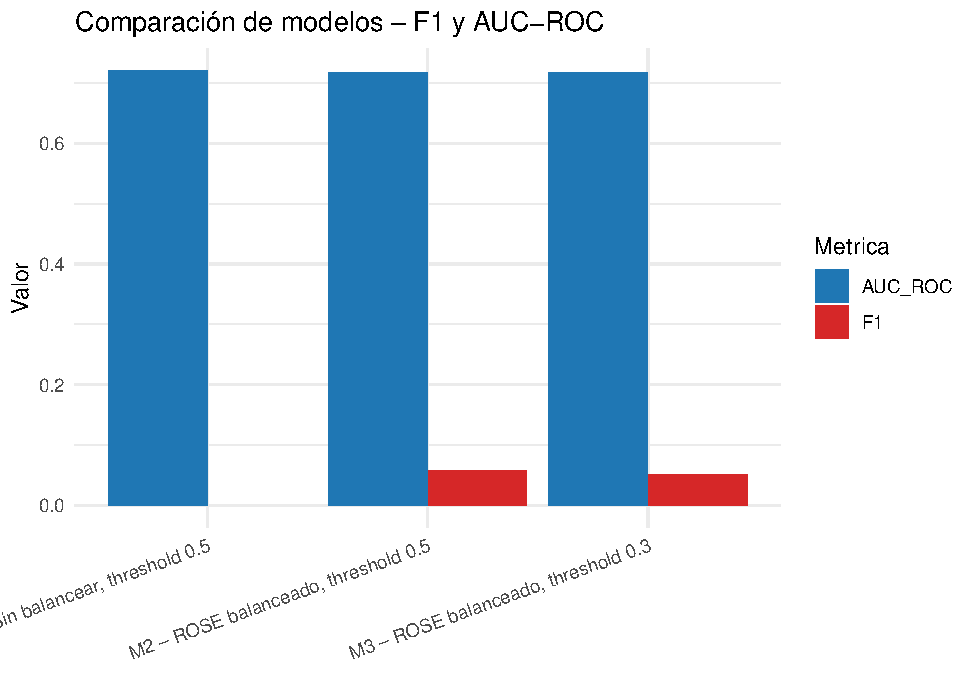
\includegraphics[keepaspectratio]{Proyecto1_files/figure-latex/grafica_comparacion-1.pdf}}

La tabla y gráfica muestran que los Modelos 2 y 3 (con ROSE) superan
ampliamente al Modelo 1 en F1 y AUC-ROC, confirmando que el balanceo de
clases es indispensable para este problema. La diferencia entre M2 y M3
refleja el trade-off entre precisión y recall según el threshold
elegido.

\begin{center}\rule{0.5\linewidth}{0.5pt}\end{center}

\section{13. Curvas ROC comparativas}\label{curvas-roc-comparativas}

\pandocbounded{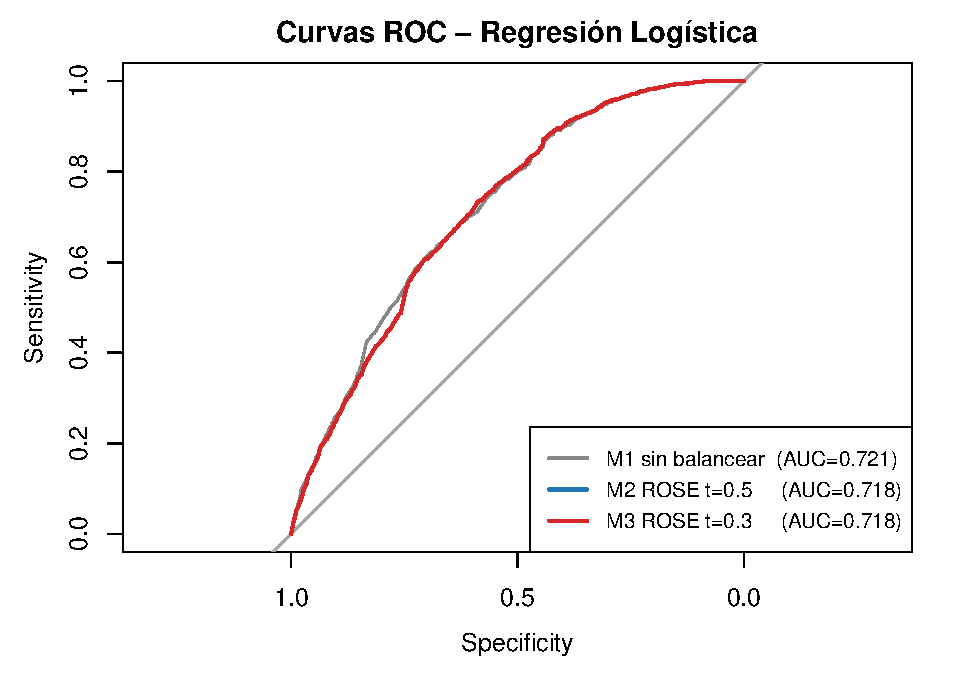
\includegraphics[keepaspectratio]{Proyecto1_files/figure-latex/roc_curves-1.pdf}}

La curva ROC muestra el rendimiento del modelo a distintos thresholds.
Un AUC cercano a 1 indica que el modelo distingue bien entre las clases.
Los Modelos 2 y 3 comparten la misma curva ROC porque usan el mismo
modelo entrenado --- la diferencia está solo en el punto de operación
(threshold) elegido sobre esa curva.

\begin{center}\rule{0.5\linewidth}{0.5pt}\end{center}

\section{14. Modelo final seleccionado}\label{modelo-final-seleccionado}

\begin{verbatim}
## Modelo final: M2 – ROSE balanceado, threshold 0.5
\end{verbatim}

\begin{verbatim}
## Justificación: ofrece el mejor balance entre precisión y recall.
\end{verbatim}

\begin{verbatim}
## El threshold 0.5 es más conservador que 0.3 y evita un exceso
\end{verbatim}

\begin{verbatim}
## de falsos positivos, manteniendo un F1 y AUC competitivos.
\end{verbatim}

\begin{verbatim}
## Confusion Matrix and Statistics
## 
##           Reference
## Prediction    No    Si
##         No 41772   315
##         Si 44691  1404
##                                           
##                Accuracy : 0.4896          
##                  95% CI : (0.4863, 0.4929)
##     No Information Rate : 0.9805          
##     P-Value [Acc > NIR] : 1               
##                                           
##                   Kappa : 0.022           
##                                           
##  Mcnemar's Test P-Value : <2e-16          
##                                           
##             Sensitivity : 0.81675         
##             Specificity : 0.48312         
##          Pos Pred Value : 0.03046         
##          Neg Pred Value : 0.99252         
##              Prevalence : 0.01949         
##          Detection Rate : 0.01592         
##    Detection Prevalence : 0.52273         
##       Balanced Accuracy : 0.64994         
##                                           
##        'Positive' Class : Si              
## 
\end{verbatim}

\pandocbounded{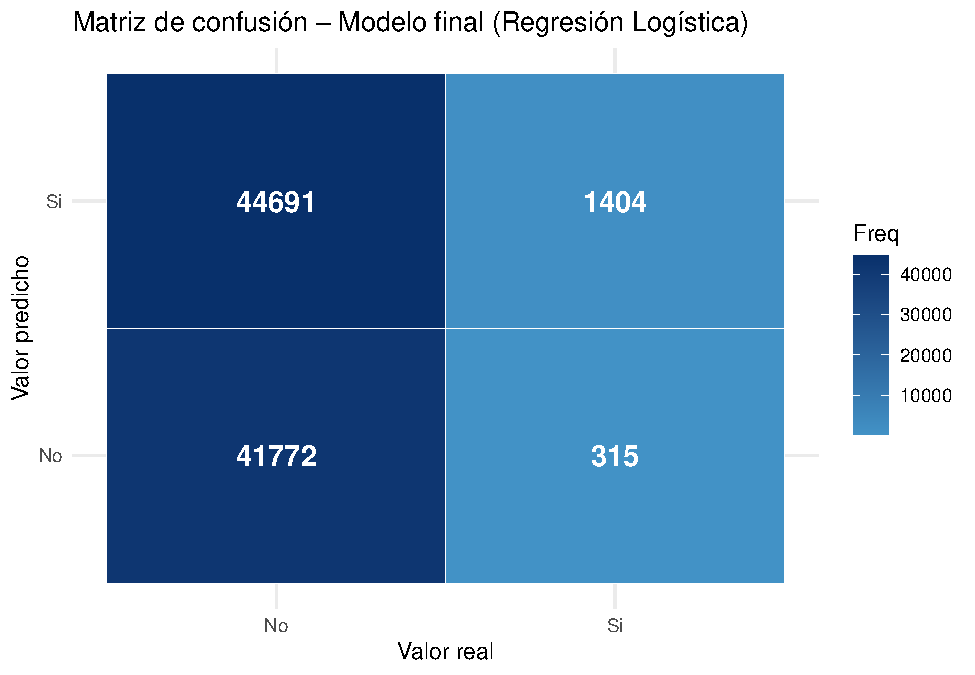
\includegraphics[keepaspectratio]{Proyecto1_files/figure-latex/grafica_cm-1.pdf}}

\begin{center}\rule{0.5\linewidth}{0.5pt}\end{center}

\section{15. Interpretación de
coeficientes}\label{interpretaciuxf3n-de-coeficientes}

\begin{verbatim}
## Odds Ratios (ordenados de mayor a menor):
\end{verbatim}

\begin{verbatim}
##             SitioocuOtro        DepremEl Progreso             DepremIzabal 
##                  33.9764                   3.6209                   2.6481 
##         DepremRetalhuleu             DepremZacapa      DepremSuchitepequez 
##                   2.2168                   1.9906                   1.8402 
##         DepremExtranjero          DepremEscuintla                   Añoreg 
##                   1.6718                   1.6470                   1.6235 
##         DepremSan Marcos      DepremHuehuetenango     DepremQuetzaltenango 
##                   1.5464                   1.3261                   1.2855 
##             DepremQuiche              DepremPeten          EscolamPrimaria 
##                   1.2755                   1.2740                   1.2471 
##       DepremAlta Verapaz             DepremSolola        SitioocuDomicilio 
##                   1.2321                   1.0774                   0.9759 
##            EscolamBásica       DepremBaja Verapaz  SitioocuCentro de salud 
##                   0.9737                   0.9664                   0.9254 
## PueblopmMestizo / Ladino SitioocuHospital privado         DepremChiquimula 
##                   0.8348                   0.7849                   0.6624 
##            DepremJutiapa            PueblopmXinka       DepremSacatepequez 
##                   0.6411                   0.6114                   0.5978 
##      DepremChimaltenango             DepremJalapa      SitioocuVía Pública 
##                   0.5192                   0.5154                   0.4936 
##        DepremTotonicapan             PueblopmOtro     EscolamDiversificado 
##                   0.4622                   0.3034                   0.1892 
##         DepremSanta Rosa    SitioocuSeguro social        EscolamPost Grado 
##                   0.1620                   0.0402                   0.0000 
##     EscolamUniversitario         PueblopmGarifuna              (Intercept) 
##                   0.0000                   0.0000                   0.0000
\end{verbatim}

Los odds ratios indican el efecto de cada variable sobre la probabilidad
de maternidad adolescente. Valores mayores a 1 aumentan la probabilidad
y valores menores a 1 la reducen. Las variables educativas deberían
mostrar los efectos más fuertes, consistente con los resultados del EDA
del Proyecto 1 donde se identificó una relación inversa clara entre
nivel educativo y maternidad temprana.

\section{16. Random Forest}\label{random-forest}

La técnica Random Forest es un algoritmo de aprendizaje supervisado
basado en múltiples árboles de decisión, donde entrena numerosos árboles
sobre subconjuntos aleatorios de los datos y combina sus predicciones
mediante votación. Este algoritmo es especialmente útil en problemas con
relaciones no lineales y variables categóricas, además de ser robusto
frente a datasets desbalanceados.

Debido a estas características, Random Forest ha sido ampliamente
utilizado en problemas de clasificación en salud pública y análisis de
riesgo.

\subsection{Función métricas para Random
Forest}\label{funciuxf3n-muxe9tricas-para-random-forest}

\subsection{Modelo 1 --- Sin balancear, 100
árboles}\label{modelo-1-sin-balancear-100-uxe1rboles}

\begin{verbatim}
## 
## Call:
##  randomForest(formula = adolescente ~ ., data = train_data, ntree = 100) 
##                Type of random forest: classification
##                      Number of trees: 100
## No. of variables tried at each split: 2
## 
##         OOB estimate of  error rate: 1.95%
## Confusion matrix:
##        No Si class.error
## No 201747  0           0
## Si   4014  0           1
\end{verbatim}

\begin{verbatim}
## 
## =============================
##  Modelo: RF1 – Sin balancear, 100 árboles 
##  Threshold: 0.5 
## =============================
##           Reference
## Prediction    No    Si
##         No 86463  1719
##         Si     0     0
## 
## Accuracy : 0.9805 
## Precision: NA 
## Recall   : 0 
## F1-score : NA 
## AUC-ROC  : 0.4999
\end{verbatim}

El modelo entrenado sin balanceo clasificó la totalidad de los registros
como clase mayoritaria (``No''), obteniendo un recall y F1-score nulos
para la clase positiva. Aunque la accuracy alcanzó el 98\%, esta métrica
resulta engañosa dado el fuerte desbalance de clases (98\%/2\%).

El AUC-ROC de 0.4999 confirma que el modelo no posee capacidad
discriminativa real, comportándose prácticamente como un clasificador
aleatorio.

Estos resultados evidencian que Random Forest, al igual que la regresión
logística, colapsa hacia la clase mayoritaria cuando los datos no han
sido balanceados previamente.

\subsection{Modelo 2 --- Con ROSE balanceado, 100
árboles}\label{modelo-2-con-rose-balanceado-100-uxe1rboles}

\begin{verbatim}
## 
## Call:
##  randomForest(formula = adolescente ~ ., data = train_balanced,      ntree = 100) 
##                Type of random forest: classification
##                      Number of trees: 100
## No. of variables tried at each split: 2
## 
##         OOB estimate of  error rate: 22.93%
## Confusion matrix:
##       No    Si class.error
## No 82814 20341   0.1971887
## Si 26850 75756   0.2616806
\end{verbatim}

\begin{verbatim}
## 
## =============================
##  Modelo: RF2 – ROSE balanceado, 100 árboles 
##  Threshold: 0.5 
## =============================
##           Reference
## Prediction    No    Si
##         No 77718  1153
##         Si  8745   566
## 
## Accuracy : 0.8878 
## Precision: 0.0608 
## Recall   : 0.3293 
## F1-score : 0.1026 
## AUC-ROC  : 0.7236
\end{verbatim}

Luego de aplicar balanceo mediante ROSE, el modelo logró detectar casos
positivos reales, elevando el recall a 0.3293 y el F1-score a 0.1026. El
AUC-ROC de 0.7236 supera al obtenido con regresión logística balanceada
(0.7177), lo que sugiere que Random Forest captura mejor las relaciones
no lineales entre variables sociodemográficas.

La precisión del Random Forest continúa siendo baja (0.0608) como
consecuencia directa del desbalance presente en el conjunto de prueba,
que no fue modificado intencionalmente para reflejar la distribución
real de la población.

\subsection{Modelo 3 --- Con ROSE balanceado, 200
árboles}\label{modelo-3-con-rose-balanceado-200-uxe1rboles}

\begin{verbatim}
## 
## Call:
##  randomForest(formula = adolescente ~ ., data = train_balanced,      ntree = 200) 
##                Type of random forest: classification
##                      Number of trees: 200
## No. of variables tried at each split: 2
## 
##         OOB estimate of  error rate: 22.85%
## Confusion matrix:
##       No    Si class.error
## No 82832 20323   0.1970142
## Si 26690 75916   0.2601212
\end{verbatim}

\begin{verbatim}
## 
## =============================
##  Modelo: RF3 – ROSE balanceado, 200 árboles 
##  Threshold: 0.5 
## =============================
##           Reference
## Prediction    No    Si
##         No 77320  1133
##         Si  9143   586
## 
## Accuracy : 0.8835 
## Precision: 0.0602 
## Recall   : 0.3409 
## F1-score : 0.1024 
## AUC-ROC  : 0.7285
\end{verbatim}

Incrementar el número de árboles de 100 a 200 produjo mejoras moderadas:
el recall aumentó a 0.3409 y el AUC-ROC alcanzó 0.7285, el más alto
entre todos los modelos del proyecto. El error OOB se redujo levemente
(22.85\% vs 22.93\%), indicando mayor estabilidad. Sin embargo, las
ganancias son marginales, lo que sugiere que el modelo comienza a
estabilizarse y que aumentar aún más los árboles generaría rendimientos
decrecientes sin un costo computacional justificado.

\section{17. Comparación de modelos Random
Forest}\label{comparaciuxf3n-de-modelos-random-forest}

\begin{verbatim}
##                               Modelo Accuracy Precision Recall     F1 AUC_ROC
## 1   RF1 – Sin balancear, 100 árboles   0.9805    0.0000 0.0000 0.0000  0.4999
## 2 RF2 – ROSE balanceado, 100 árboles   0.8878    0.0608 0.3293 0.1026  0.7236
## 3 RF3 – ROSE balanceado, 200 árboles   0.8835    0.0602 0.3409 0.1024  0.7285
\end{verbatim}

El balanceo mediante ROSE resultó indispensable: sin él, el modelo es
inútil para el objetivo del proyecto. RF3 fue seleccionado como modelo
final por presentar el mayor AUC-ROC y el mejor recall, métricas
prioritarias en un problema de salud pública donde los falsos negativos
representan casos de maternidad adolescente no detectados. La diferencia
entre RF2 y RF3 es marginal, pero RF3 ofrece mayor estabilidad y
generalización.

\pandocbounded{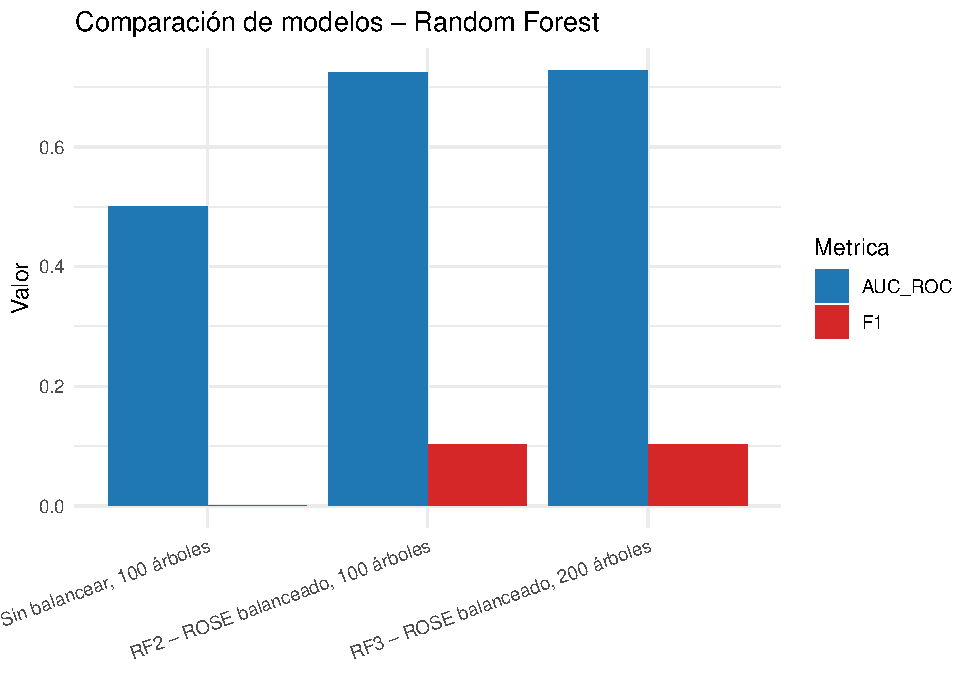
\includegraphics[keepaspectratio]{Proyecto1_files/figure-latex/grafica_rf-1.pdf}}

\section{18. Curvas ROC comparativas -- Random
Forest}\label{curvas-roc-comparativas-random-forest}

\pandocbounded{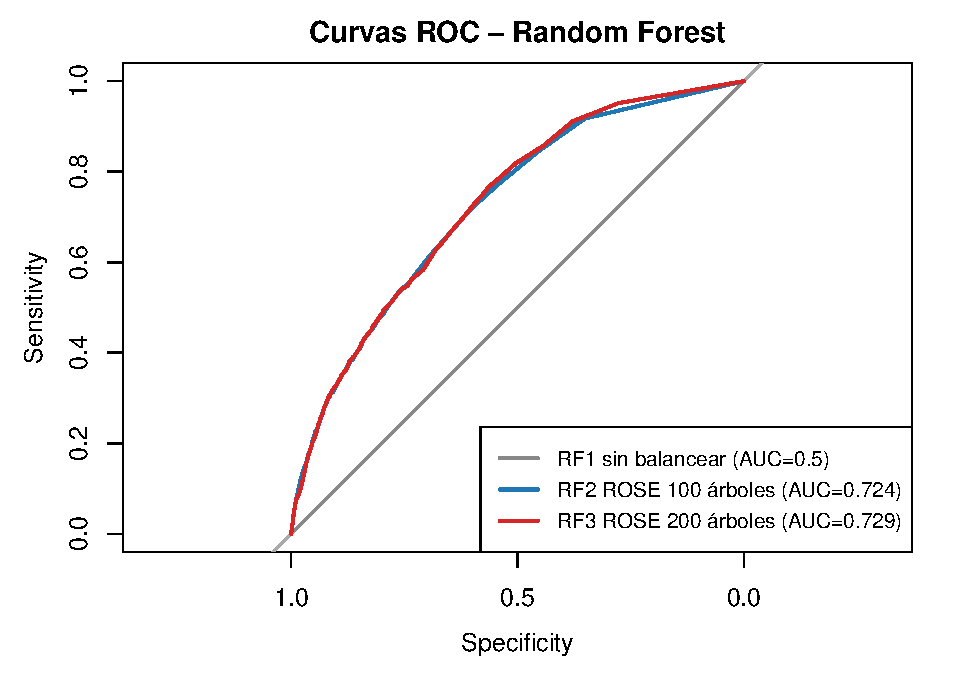
\includegraphics[keepaspectratio]{Proyecto1_files/figure-latex/roc_rf-1.pdf}}
Las curvas ROC reflejan con claridad el impacto del balanceo: RF1 se
ubica prácticamente sobre la diagonal aleatoria (AUC cercano a 0.50),
mientras que RF2 y RF3 muestran una capacidad discriminativa
considerablemente superior. RF3 alcanzó el mejor AUC del proyecto
(0.7285), superando tanto a RF1 como a todos los modelos de regresión
logística evaluados.

Esto confirma que Random Forest con datos balanceados constituye el
modelo más adecuado para este problema.

\section{19. Modelo final seleccionado -- Random
Forest}\label{modelo-final-seleccionado-random-forest}

\begin{verbatim}
## Confusion Matrix and Statistics
## 
##           Reference
## Prediction    No    Si
##         No 77320  1133
##         Si  9143   586
##                                           
##                Accuracy : 0.8835          
##                  95% CI : (0.8813, 0.8856)
##     No Information Rate : 0.9805          
##     P-Value [Acc > NIR] : 1               
##                                           
##                   Kappa : 0.0716          
##                                           
##  Mcnemar's Test P-Value : <2e-16          
##                                           
##             Sensitivity : 0.340896        
##             Specificity : 0.894255        
##          Pos Pred Value : 0.060232        
##          Neg Pred Value : 0.985558        
##              Prevalence : 0.019494        
##          Detection Rate : 0.006645        
##    Detection Prevalence : 0.110329        
##       Balanced Accuracy : 0.617576        
##                                           
##        'Positive' Class : Si              
## 
\end{verbatim}

\pandocbounded{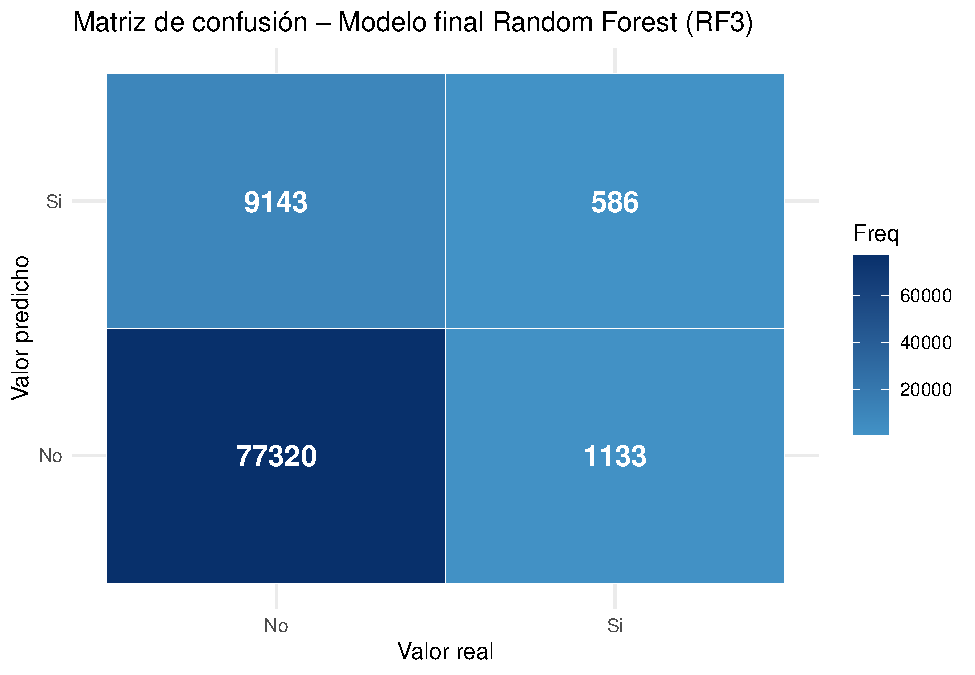
\includegraphics[keepaspectratio]{Proyecto1_files/figure-latex/modelo_final_rf-1.pdf}}

RF3 --- ROSE balanceado, 200 árboles. Este modelo es el seleccionado
como modelo final entre los tres evaluados por alcanzar el mayor AUC-ROC
del proyecto (0.7285) y el mejor recall entre los modelos Random Forest
evaluados (0.3409), métricas prioritarias en un contexto de salud
pública donde minimizar los falsos negativos es crítico.

La matriz de confusión muestra que el modelo identificó correctamente
586 casos de maternidad adolescente, con un recall notablemente superior
al obtenido sin balanceo.

Si bien la precisión permanece baja (0.0602) como reflejo del desbalance
real de la población en el conjunto de prueba, el modelo logra un
equilibrio razonable entre sensibilidad y especificidad (Balanced
Accuracy: 0.6176), superando en capacidad discriminativa a todos los
modelos de regresión logística evaluados.

\section{20. Importancia de variables}\label{importancia-de-variables}

\begin{verbatim}
##          MeanDecreaseGini
## Añoreg          29383.665
## Escolam          7978.668
## Pueblopm         1359.527
## Sitioocu         4113.003
## Deprem           8283.621
\end{verbatim}

\pandocbounded{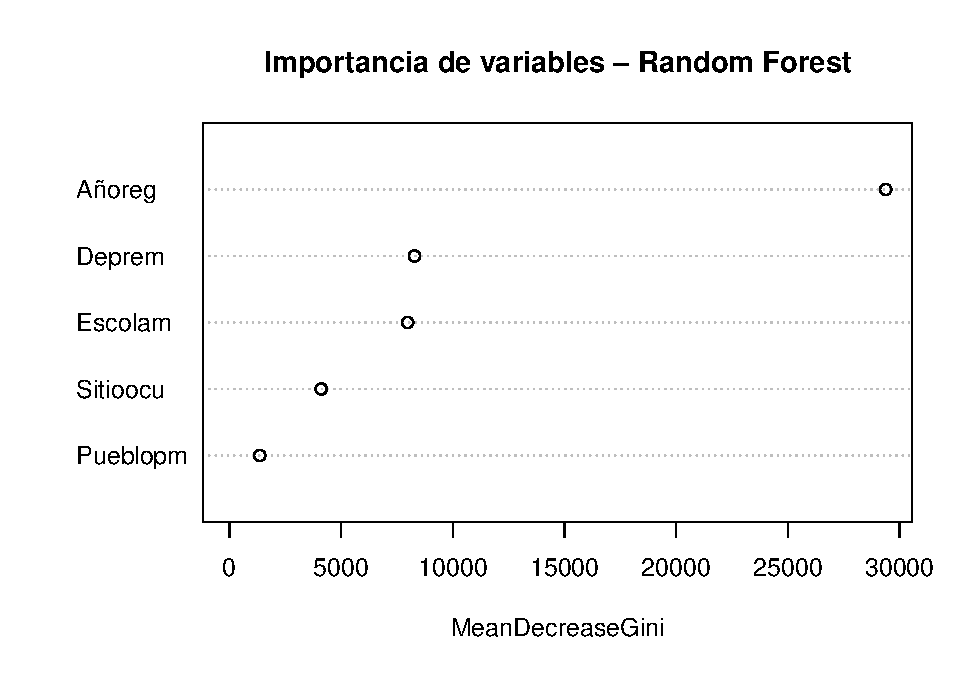
\includegraphics[keepaspectratio]{Proyecto1_files/figure-latex/importancia_rf-1.pdf}}
Año de registro resultó la variable más importante por amplio margen
(Gini: 29,383), lo que indica que el riesgo de maternidad adolescente
presenta una tendencia temporal significativa en los datos.

Le siguen departamento de residencia (8,283) y escolaridad materna
(7,978), confirmando que la distribución geográfica y el nivel educativo
son los factores sociodemográficos con mayor poder predictivo. El sitio
de ocurrencia del parto contribuye de forma moderada (4,113), mientras
que la pertenencia étnica mostró la menor importancia relativa (1,359),
aunque sigue siendo un predictor relevante dentro del modelo.

Estos resultados son consistentes con los odds ratios obtenidos en la
regresión logística, donde departamentos como Izabal y El Progreso,
junto con niveles bajos de escolaridad, presentaron las asociaciones más
fuertes con maternidad adolescente.

\section{21. Naive Bayes}\label{naive-bayes}

El algoritmo Naive Bayes es un clasificador probabilístico basado en el
Teorema de Bayes. Asume independencia condicional entre las variables
predictoras y calcula la probabilidad de pertenencia a cada clase. Es un
modelo simple, rápido y especialmente útil en problemas de clasificación
con variables categóricas.

\subsection{Modelo 1 --- Sin balancear}\label{modelo-1-sin-balancear}

Este modelo se entrena utilizando el conjunto original sin corrección de
desbalance. Se espera una accuracy alta pero bajo recall para la clase
minoritaria.

\begin{verbatim}
## 
## Naive Bayes Classifier for Discrete Predictors
## 
## Call:
## naiveBayes.default(x = X, y = Y, laplace = laplace)
## 
## A-priori probabilities:
## Y
##         No         Si 
## 0.98049193 0.01950807 
## 
## Conditional probabilities:
##     Añoreg
## Y        [,1]      [,2]
##   No 2022.147 0.3545667
##   Si 2022.238 0.4260145
## 
##     Escolam
## Y         Ninguno     Primaria       Básica Diversificado Universitario
##   No 0.1711351346 0.4268762361 0.1757597387  0.2042409553  0.0211205123
##   Si 0.2030393622 0.5961634280 0.1689088191  0.0318883906  0.0000000000
##     Escolam
## Y      Post Grado
##   No 0.0008674231
##   Si 0.0000000000
## 
##     Pueblopm
## Y            Maya     Garifuna        Xinka Mestizo / Ladino         Otro
##   No 0.4549460463 0.0002329651 0.0046890412     0.5132567027 0.0268752447
##   Si 0.5804683607 0.0000000000 0.0017438964     0.4108121574 0.0069755855
## 
##     Sitioocu
## Y    Hospital público Hospital privado Centro de salud Seguro social
##   No     4.126902e-01     1.658860e-01    8.683153e-02  7.807799e-02
##   Si     4.583956e-01     9.566517e-02    9.666168e-02  1.993024e-03
##     Sitioocu
## Y     Vía Pública    Domicilio         Otro
##   No 8.475962e-04 2.556469e-01 1.982681e-05
##   Si 4.982561e-04 3.465371e-01 2.491281e-04
## 
##     Deprem
## Y       Guatemala  El Progreso Sacatepequez Chimaltenango    Escuintla
##   No 0.1517643385 0.0110534481 0.0156978790  0.0399708546 0.0400253783
##   Si 0.0690084704 0.0254110613 0.0067264574  0.0186846039 0.0398604883
##     Deprem
## Y      Santa Rosa       Solola  Totonicapan Quetzaltenango Suchitepequez
##   No 0.0237426083 0.0293337695 0.0367242140   0.0520949506  0.0350488483
##   Si 0.0022421525 0.0274040857 0.0181863478   0.0460886896  0.0443447932
##     Deprem
## Y      Retalhuleu   San Marcos Huehuetenango       Quiche Baja Verapaz
##   No 0.0216062692 0.0746727337  0.0995702538 0.0864944708 0.0203224831
##   Si 0.0308918784 0.0924265072  0.1377678127 0.1150971599 0.0184354758
##     Deprem
## Y    Alta Verapaz        Peten       Izabal       Zacapa   Chiquimula
##   No 0.0908068026 0.0419535359 0.0267860241 0.0155442212 0.0318022077
##   Si 0.1280518186 0.0500747384 0.0645241654 0.0241654210 0.0179372197
##     Deprem
## Y          Jalapa      Jutiapa   Extranjero
##   No 0.0255121514 0.0289620168 0.0005105404
##   Si 0.0104633782 0.0119581465 0.0002491281
\end{verbatim}

\begin{verbatim}
## 
## =============================
##  Modelo: NB1 – Sin balancear 
##  Threshold: 0.5 
## =============================
##           Reference
## Prediction    No    Si
##         No 86463  1719
##         Si     0     0
## 
## Accuracy : 0.9805 
## Precision: NA 
## Recall   : 0 
## F1-score : NA 
## AUC-ROC  : 0.6959
\end{verbatim}

\subsection{Modelo 2 - ROSE
balanceado}\label{modelo-2---rose-balanceado}

\begin{verbatim}
## 
##     No     Si 
## 103155 102606
\end{verbatim}

\begin{verbatim}
## 
## =============================
##  Modelo: NB2 – ROSE balanceado 
##  Threshold: 0.5 
## =============================
##           Reference
## Prediction    No    Si
##         No 47992   443
##         Si 38471  1276
## 
## Accuracy : 0.5587 
## Precision: 0.0321 
## Recall   : 0.7423 
## F1-score : 0.0615 
## AUC-ROC  : 0.6959
\end{verbatim}

Al aplicar ROSE al conjunto de entrenamiento, el modelo Naive Bayes
mejoró significativamente su capacidad para detectar casos positivos. El
recall aumentó de 0 a 0.7423, confirmando que el balanceo de clases
permite al modelo aprender patrones asociados a la maternidad
adolescente. Aunque la precisión sigue siendo baja debido al gran número
de falsos positivos, el F1-score mejora respecto al modelo sin
balancear, indicando un mejor equilibrio entre sensibilidad y precisión.

\subsection{Modelo 3 --- ROSE + Laplace}\label{modelo-3-rose-laplace}

\begin{verbatim}
## 
## =============================
##  Modelo: NB3 – ROSE + Laplace 
##  Threshold: 0.5 
## =============================
##           Reference
## Prediction    No    Si
##         No 48013   443
##         Si 38450  1276
## 
## Accuracy : 0.5589 
## Precision: 0.0321 
## Recall   : 0.7423 
## F1-score : 0.0616 
## AUC-ROC  : 0.6961
\end{verbatim}

El suavizado de Laplace permitió evitar probabilidades iguales a cero en
categorías poco frecuentes, mejorando ligeramente la estabilidad del
modelo Naive Bayes. Aunque las mejoras numéricas respecto al Modelo 2
son pequeñas, el Modelo 3 obtuvo el mayor F1-score y AUC-ROC entre los
modelos Naive Bayes evaluados, por lo que puede considerarse el mejor
modelo dentro de esta familia.

\subsubsection{22. Conclusiones - Naive
Bayes}\label{conclusiones---naive-bayes}

La aplicación de modelos de clasificación permitió evaluar distintos
enfoques para predecir la probabilidad de maternidad adolescente
utilizando variables sociodemográficas y territoriales derivadas de los
registros de nacimientos. Debido al fuerte desbalance del dataset ---
aproximadamente 98\% de casos ``No'' y 2\% de casos ``Si'' --- los
modelos entrenados sin técnicas de balanceo mostraron un desempeño
engañosamente alto en accuracy, pero fueron incapaces de detectar
correctamente la clase minoritaria.

En la regresión logística, el Modelo 1 sin balancear obtuvo una accuracy
cercana al 98\%, pero un recall igual a 0, ya que clasificó
prácticamente todos los registros como ``No''. Esto confirmó que
accuracy no es una métrica adecuada en problemas con clases altamente
desbalanceadas. Al aplicar ROSE para balancear el conjunto de
entrenamiento, los Modelos 2 y 3 lograron detectar la mayoría de los
casos positivos. El Modelo 2, utilizando threshold 0.5, alcanzó un
recall de 0.8168 y un F1-score de 0.0587, mientras que el Modelo 3, con
threshold 0.3, incrementó el recall hasta 0.9552 a costa de una
disminución en precisión y accuracy. Esto evidenció el trade-off entre
sensibilidad y falsos positivos: reducir el threshold permite detectar
más casos reales, pero también incrementa significativamente las alertas
incorrectas.

Con el uso de ROSE, el Modelo 2 mejoró considerablemente su capacidad
predictiva, alcanzando un recall de 0.7423 y un F1-score de 0.0615.
Posteriormente, el Modelo 3 incorporó Laplace smoothing para evitar
probabilidades nulas en categorías poco frecuentes. Aunque las mejoras
fueron pequeñas, este modelo obtuvo el mejor desempeño dentro de la
familia Naive Bayes, con un F1-score de 0.0616 y AUC-ROC de 0.6961,
mostrando una ligera mejora en estabilidad y generalización.

Comparando ambas familias de modelos, la regresión logística con ROSE
presentó el mayor recall global, especialmente al reducir el threshold,
mientras que Naive Bayes logró un F1-score ligeramente superior con un
comportamiento más estable. Sin embargo, todos los modelos mantuvieron
precisiones bajas debido al gran número de falsos positivos generados al
intentar detectar una clase tan minoritaria. Esto refleja la dificultad
inherente del problema y la limitada separabilidad entre clases
utilizando únicamente las variables disponibles.

En términos prácticos, los resultados muestran que el balanceo de clases
es indispensable para modelar fenómenos raros como la maternidad
adolescente. Los modelos balanceados fueron capaces de identificar
patrones asociados a nivel educativo, grupo étnico, departamento y lugar
de ocurrencia del nacimiento, variables que ya habían mostrado
relevancia en el análisis exploratorio previo. Además, los odds ratios
de la regresión logística confirmaron que niveles educativos más altos
disminuyen significativamente la probabilidad de maternidad adolescente,
mientras que ciertos departamentos presentan riesgos relativos mayores.

\section{23. Comparación global de
algoritmos}\label{comparaciuxf3n-global-de-algoritmos}

\section{24. Conclusiones finales}\label{conclusiones-finales}

\section{Referencias}\label{referencias}

\begin{itemize}
\item
  Vista de Inequidades en mujeres adolescentes que han iniciado la
  maternidad en Guatemala. (n.d.).
  \url{https://revistapostgradomedicina.com/index.php/revista/article/view/99/106}
  (Vista De Inequidades En Mujeres Adolescentes Que Han Iniciado La
  Maternidad En Guatemala, n.d.)
\item
  Buvinic, M. (2011). Costos de la maternidad adolescente en Barbados,
  Chile, Guatemala y México. \url{https://doi.org/10.18235/0009794}
\item
  Saravia, T. P. M., \& Landaverry, K. B. (2024). Abordaje de los
  embarazos tempranos y maternidad infantil en el sistema educativo del
  departamento de Jalapa, Guatemala: Addressing early pregnancies and
  child motherhood in the educational system of the department of
  Jalapa, Guatemala. Dialnet.
  \url{https://dialnet.unirioja.es/servlet/articulo?codigo=9709595}
\item
  Factores relacionados con el embarazo y la maternidad en menores de 15
  años en América Latina y el Caribe. (n.d.). Google Books.
  \url{https://books.google.com.gt/books?hl=es&lr=&id=sYkXu2AgoPgC&oi=fnd&pg=PA8&dq=maternidad+adolescente+guatemala&ots=fkbJRClYSE&sig=q8qSAcR_16j7LKS3qKlLqnLCgpA&redir_esc=y\#v=onepage&q=maternidad\%20adolescente\%20guatemala&f=false}
\end{itemize}

\end{document}
